\documentclass[pdf]{beamer}
\mode<presentation>{}
\usetheme{Copenhagen}
\usepackage{graphicx}
\usepackage{tabularx}

\title{Evolution of emergence strategies}
\subtitle{How organisms combine cues to make decisions}
\author{Collin Edwards 
Louie Yang}
\date{\today}

%The following adds sweet section overview slides whenever you begin a new section
\AtBeginSection[]
{
\begin{frame}{Table of Contents}
\tableofcontents[currentsection]
\end{frame}
}

\begin{document}
\begin{frame}
 \maketitle
\end{frame}
\section{Introduction}

\begin{frame}
\frametitle{}
%\begin{columns}
%\column{.6\textwidth}
%\begin{itemize}
% \item Organisms have some agency in when life history events (emergence, hatching, migrating, breeding) occur
% \item Timing of life history events matter for fitness
% \item In particular, abiotic conditions matter
% \item So\dots selection for organisms to become tiny weathermen
%\end{itemize}
%\column{.4\textwidth}
\begin{center}
\only<1>{
\begin{figure}
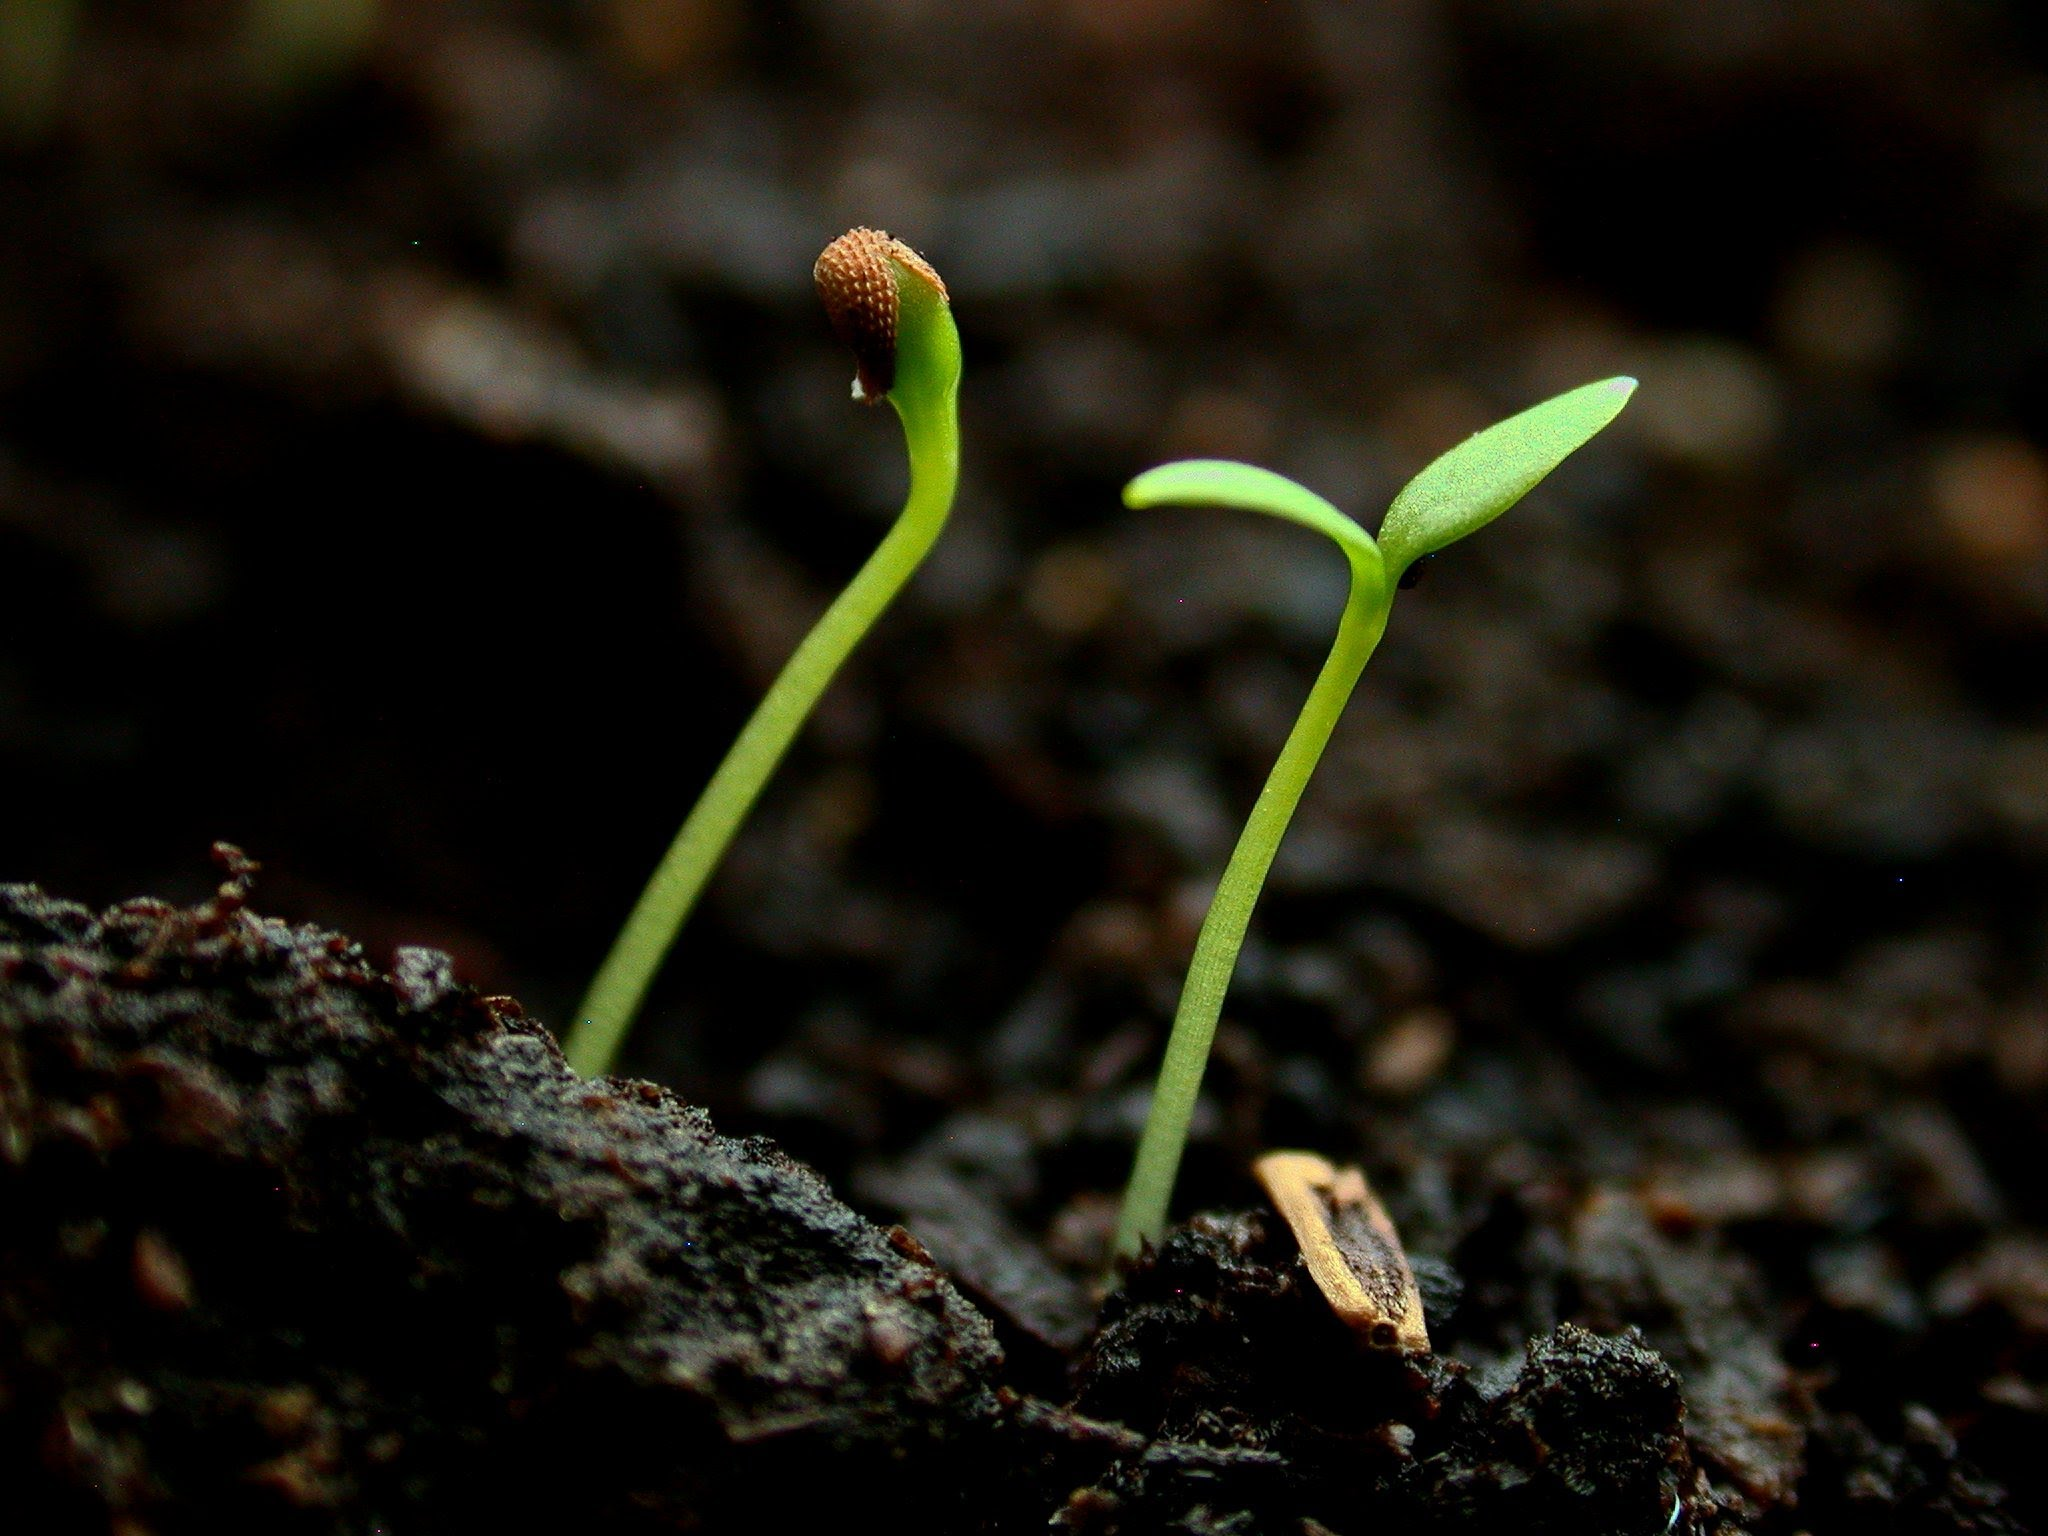
\includegraphics[width=.9\textwidth]{figs/germination.jpg}
%\caption{photo by TexasPrepper2 from youtube.com}
\end{figure}
}

\only<2>{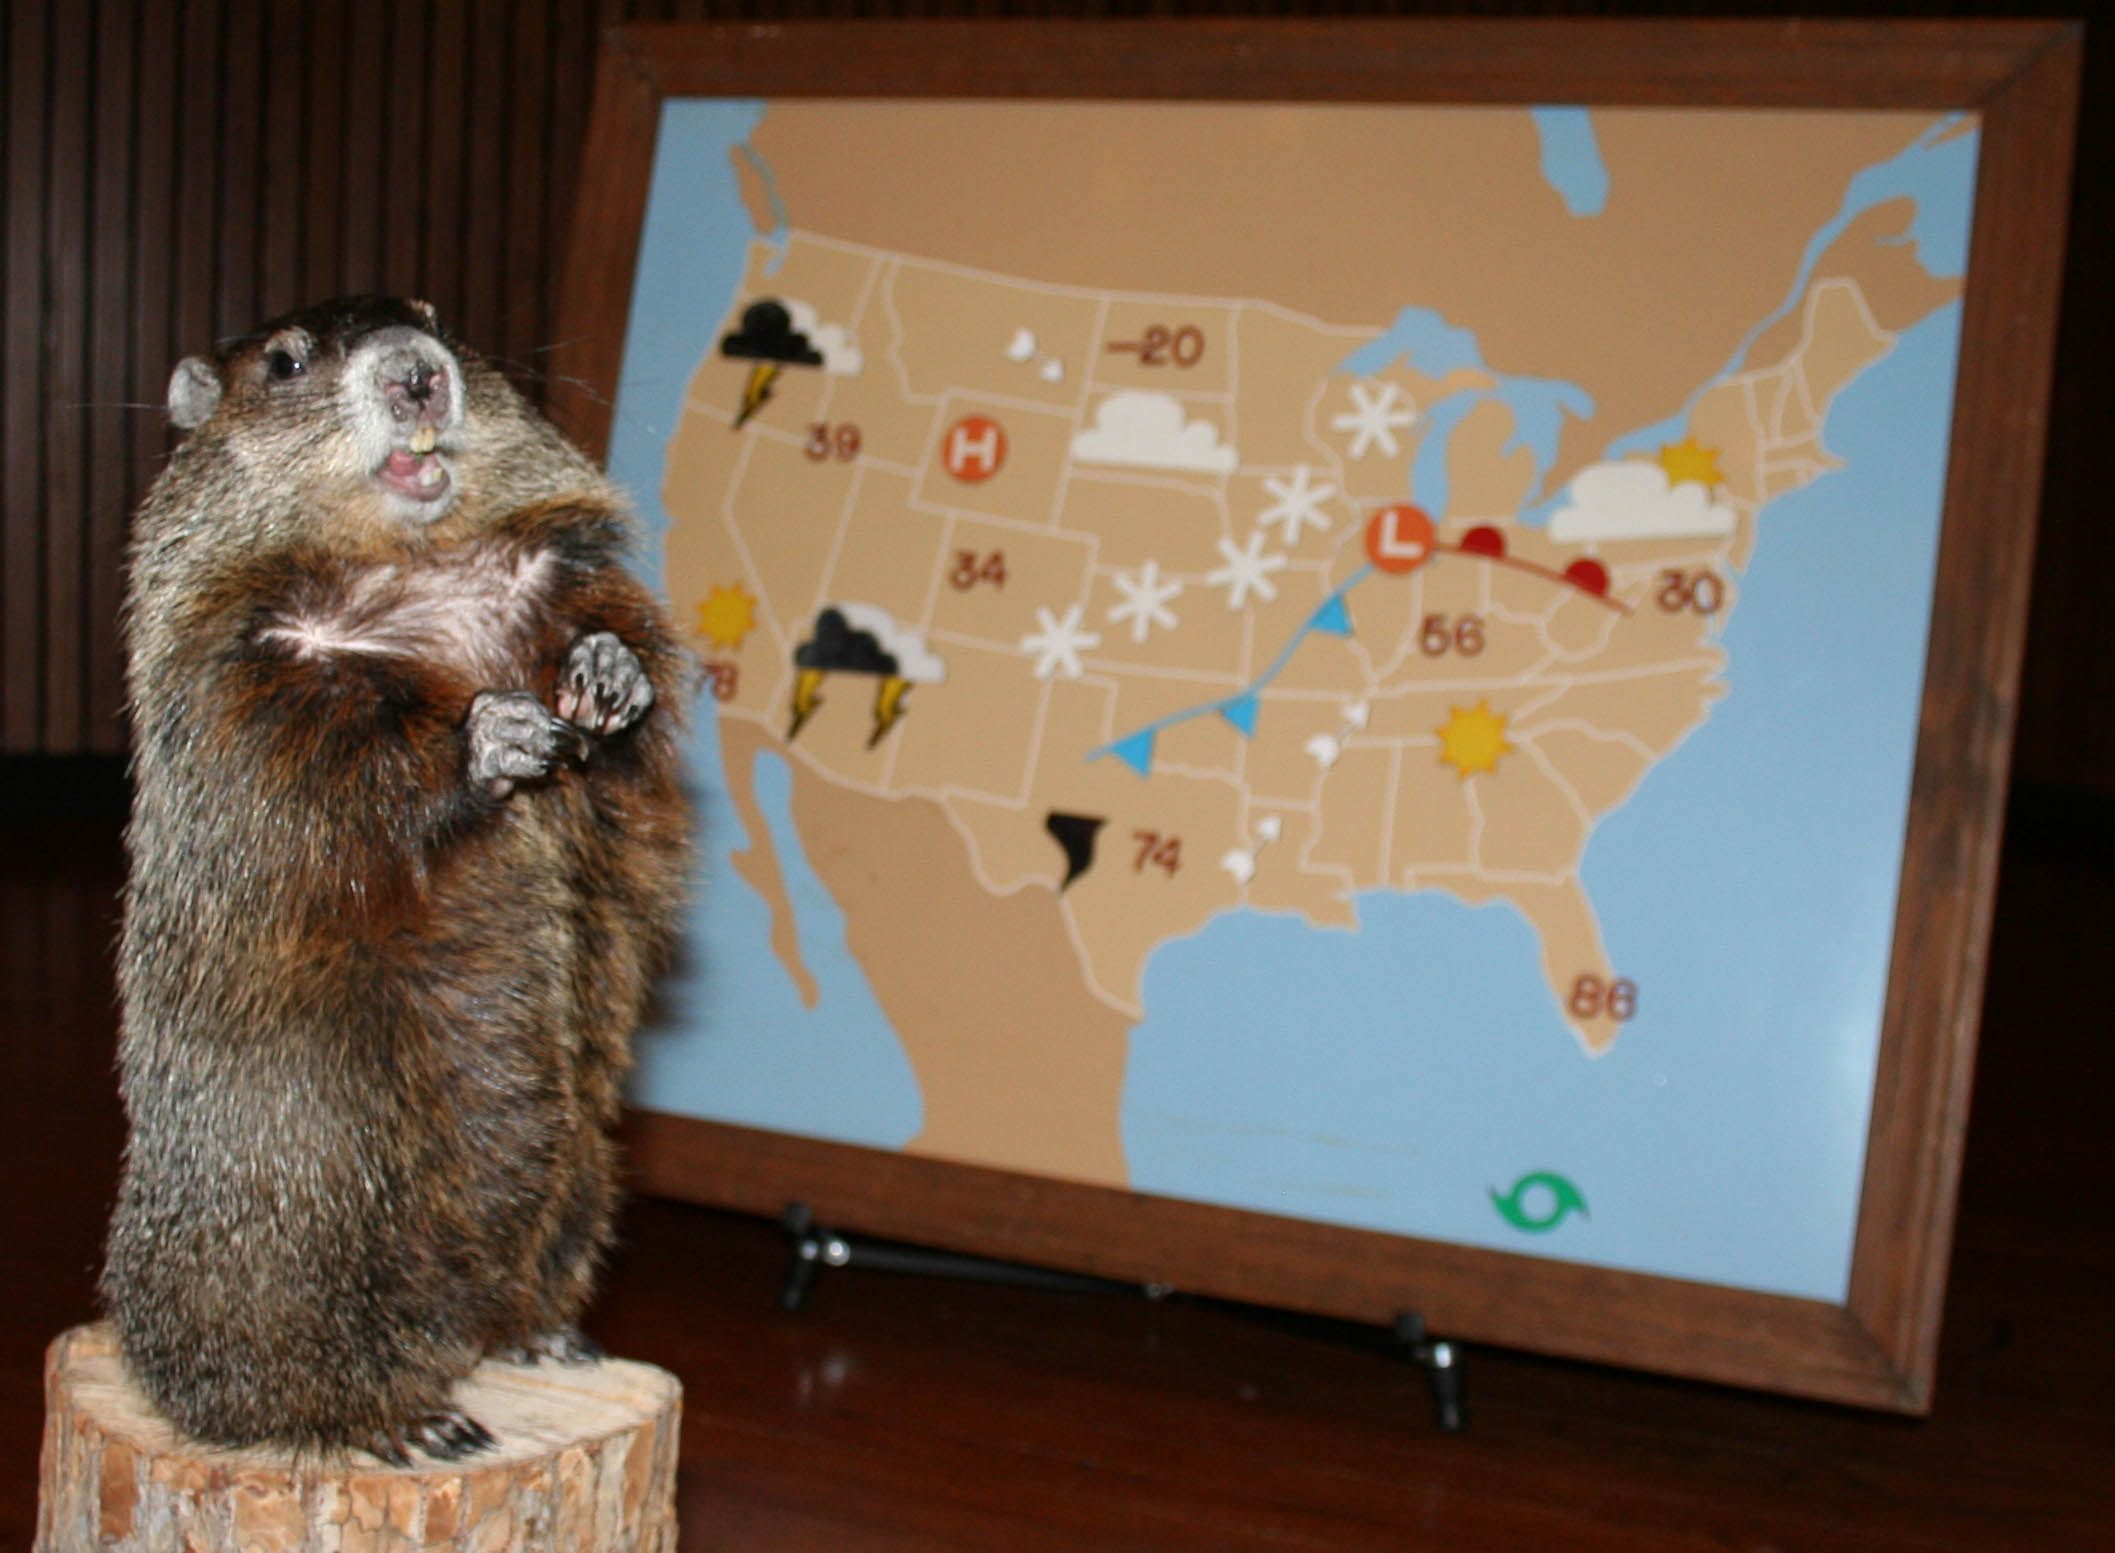
\includegraphics[width=.8\textwidth]{figs/animal-weatherman.jpg}}
\only<3>{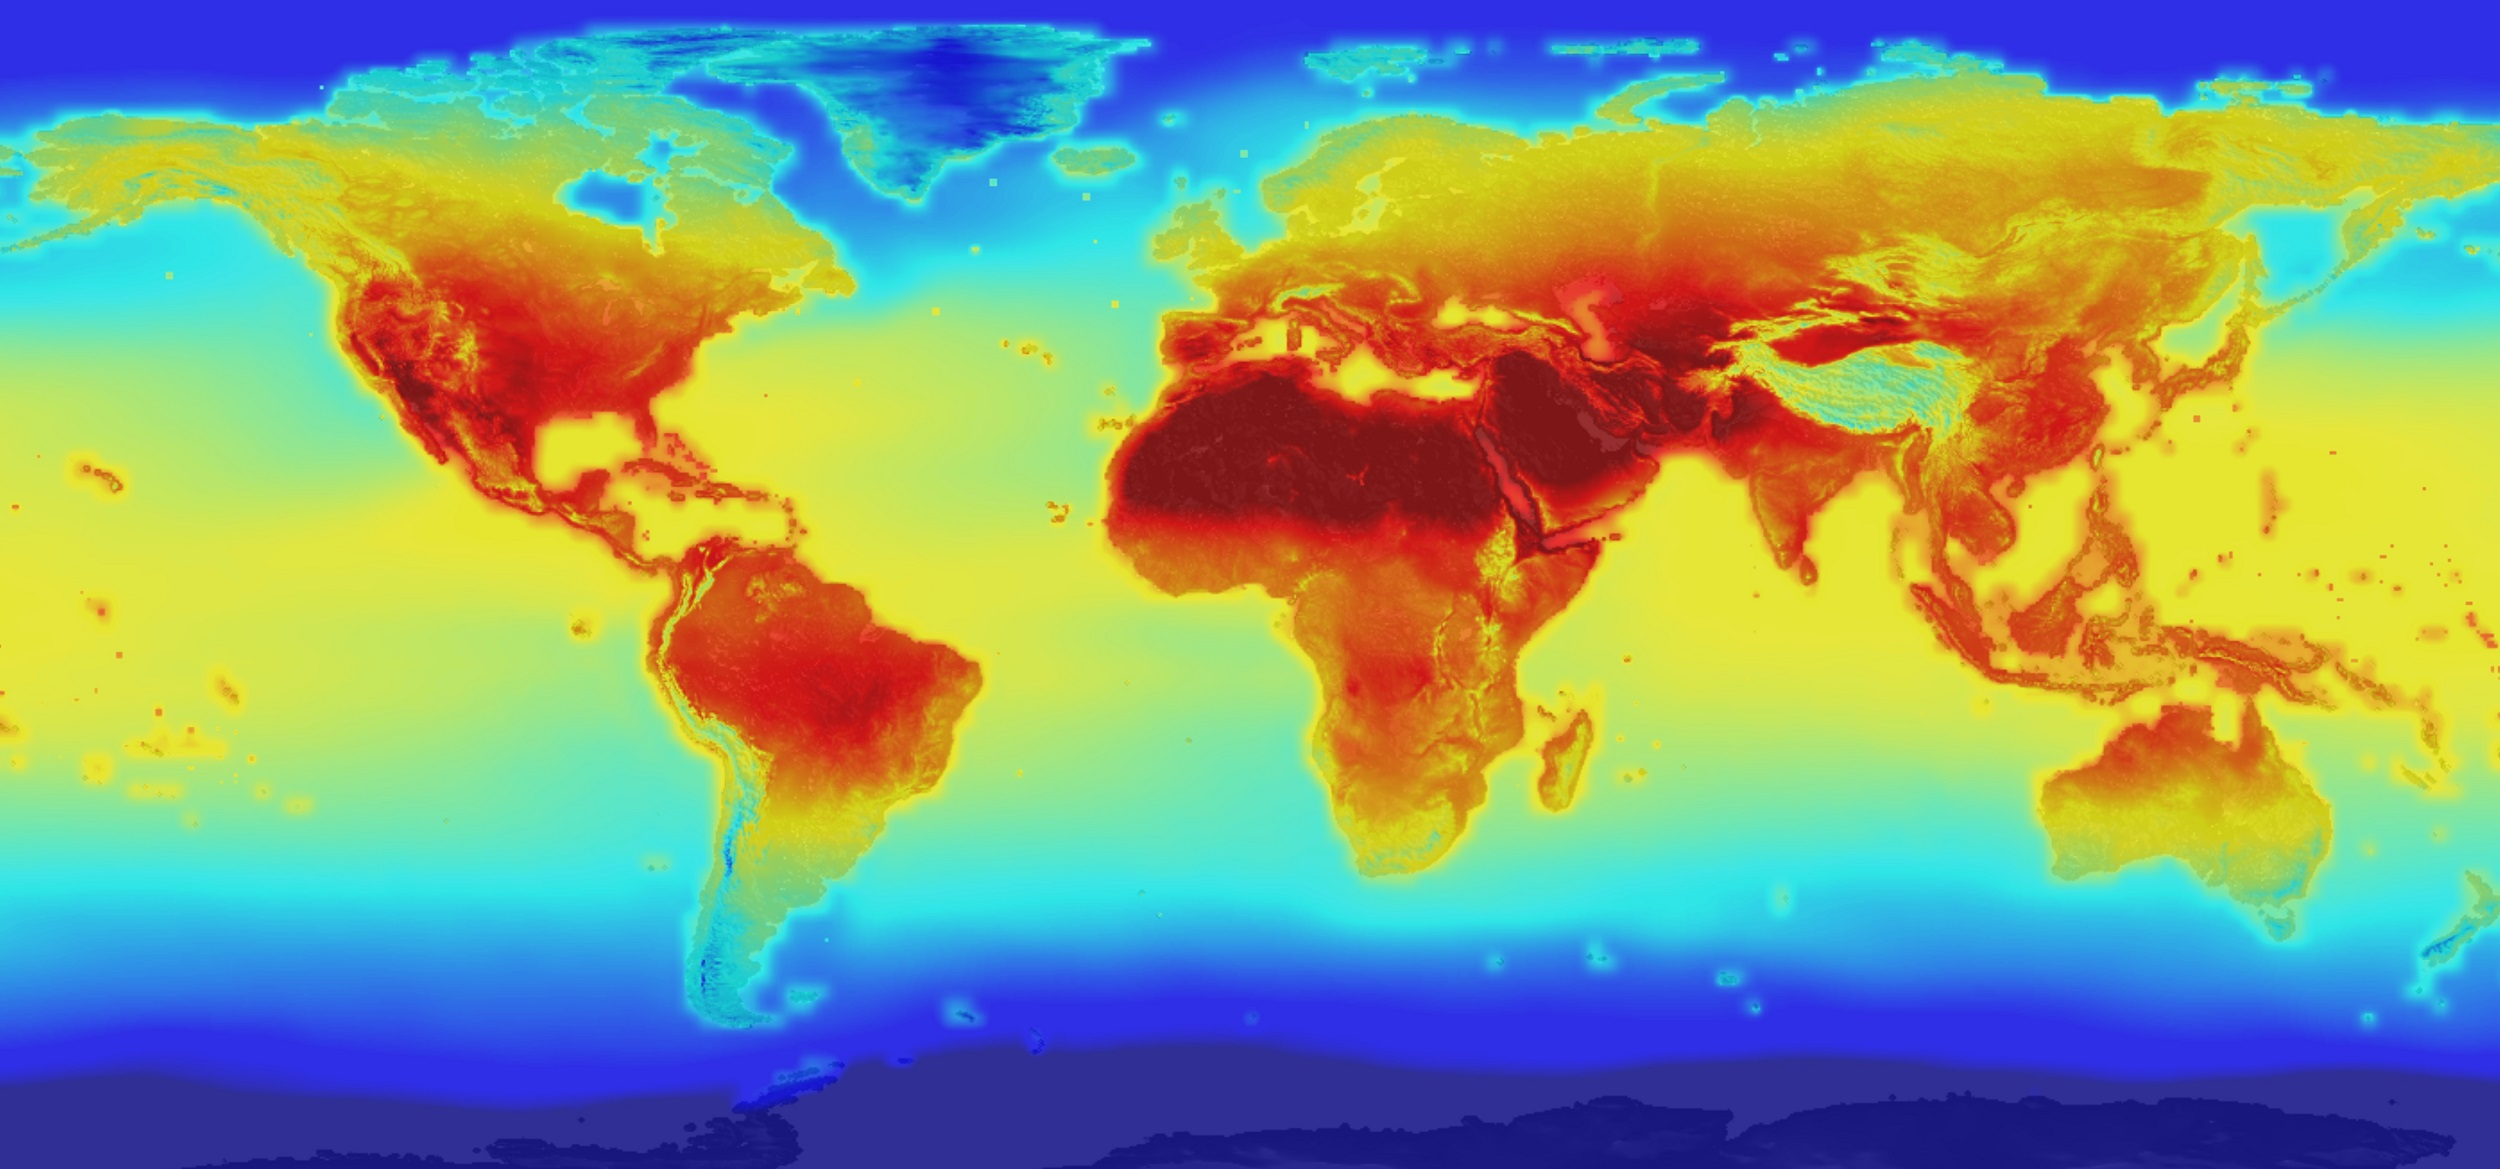
\includegraphics[width=.8\textwidth]{figs/climate-change.jpg}}
\end{center}
%\end{columns}
\end{frame}

%\begin{frame}
%\frametitle{climate change = bad}
%\begin{columns}
%\column{.6\textwidth}
%\begin{itemize}
% \item abiotic conditions are shifting
% \item many organisms must change their phenology to succeed
% \item the extent to which they're doing so is variable
%\end{itemize}
%\column{.4\textwidth}
%picture of climate change
%\end{columns}
%\end{frame}

%\begin{frame}
%\frametitle{Motivation}
%\begin{columns}
%\column{.6\textwidth}
%\begin{itemize}
% \item Broad patterns in phenology shifts? Weak/conflicting evidence
% \item little is known about phenology mechanisms
% \item expectation that organisms integrate multiple cues
%\end{itemize}
%\column{.4\textwidth}
%Picture?
%\end{columns}
%\end{frame}

\begin{frame}
\frametitle{Goals}
%\begin{columns}
%\column{.6\textwidth}
\begin{itemize}
 \item Provide base-line model for multiple-cue decisions
 \item Develop predictions for the use of phenological cues
\end{itemize}
%\column{.4\textwidth}
%Picture?
%\end{columns}
\end{frame}


\section{Simulation}
\begin{frame}
\frametitle{Basics}
%\begin{columns}
%\column{.6\textwidth}
Let's start by imagining a very simplified system:
\begin{itemize}
 \item Organisms decide when to emerge/germinate based on trait values and environmental cues \pause
 \item Organisms collect resources ($\sim$fitness) based on abiotic conditions for a set duration after emerging (10 days) \pause
 \item Lottery model reproduction: parents produce offspring proportional to resouces gathered, each offspring has equal chance of filling one of the N `slots' for adults in the next generation
\end{itemize}
%\column{.4\textwidth}
%\end{columns}
\end{frame}

\begin{frame}
\frametitle{Emergence Cues}
\begin{columns}
\column{.3\textwidth}
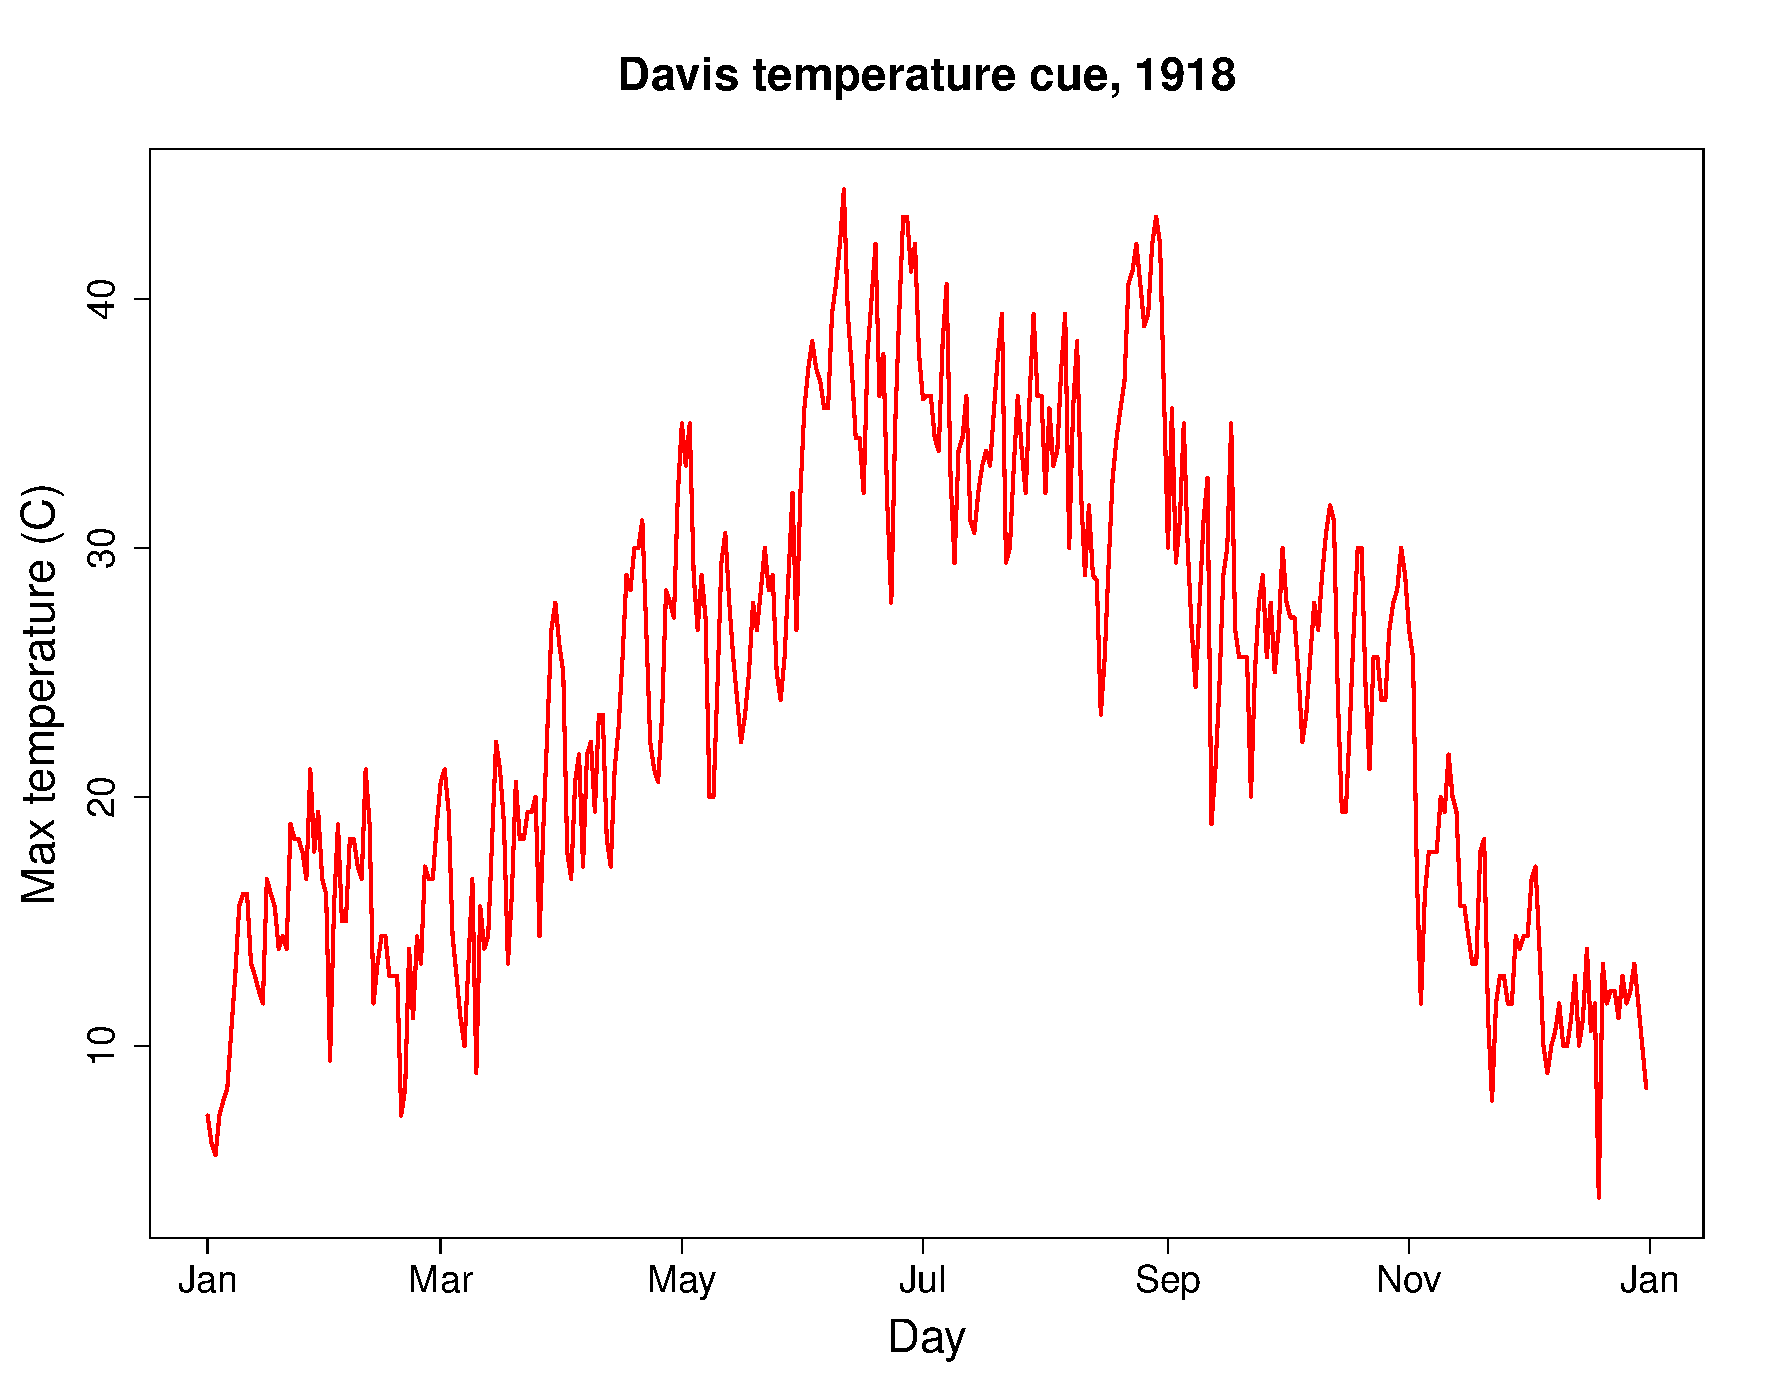
\includegraphics[width=.8\textwidth]{figs/cue-temp.pdf} \pause
\column{.3\textwidth}
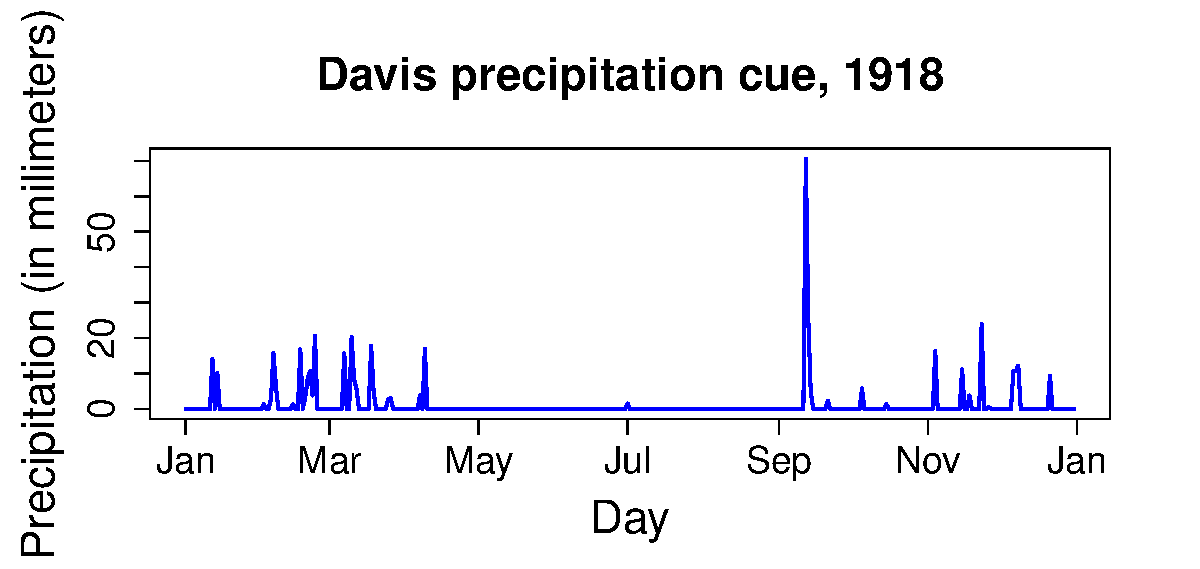
\includegraphics[width=.8\textwidth]{figs/cue-precip.pdf} \pause
\column{.3\textwidth}
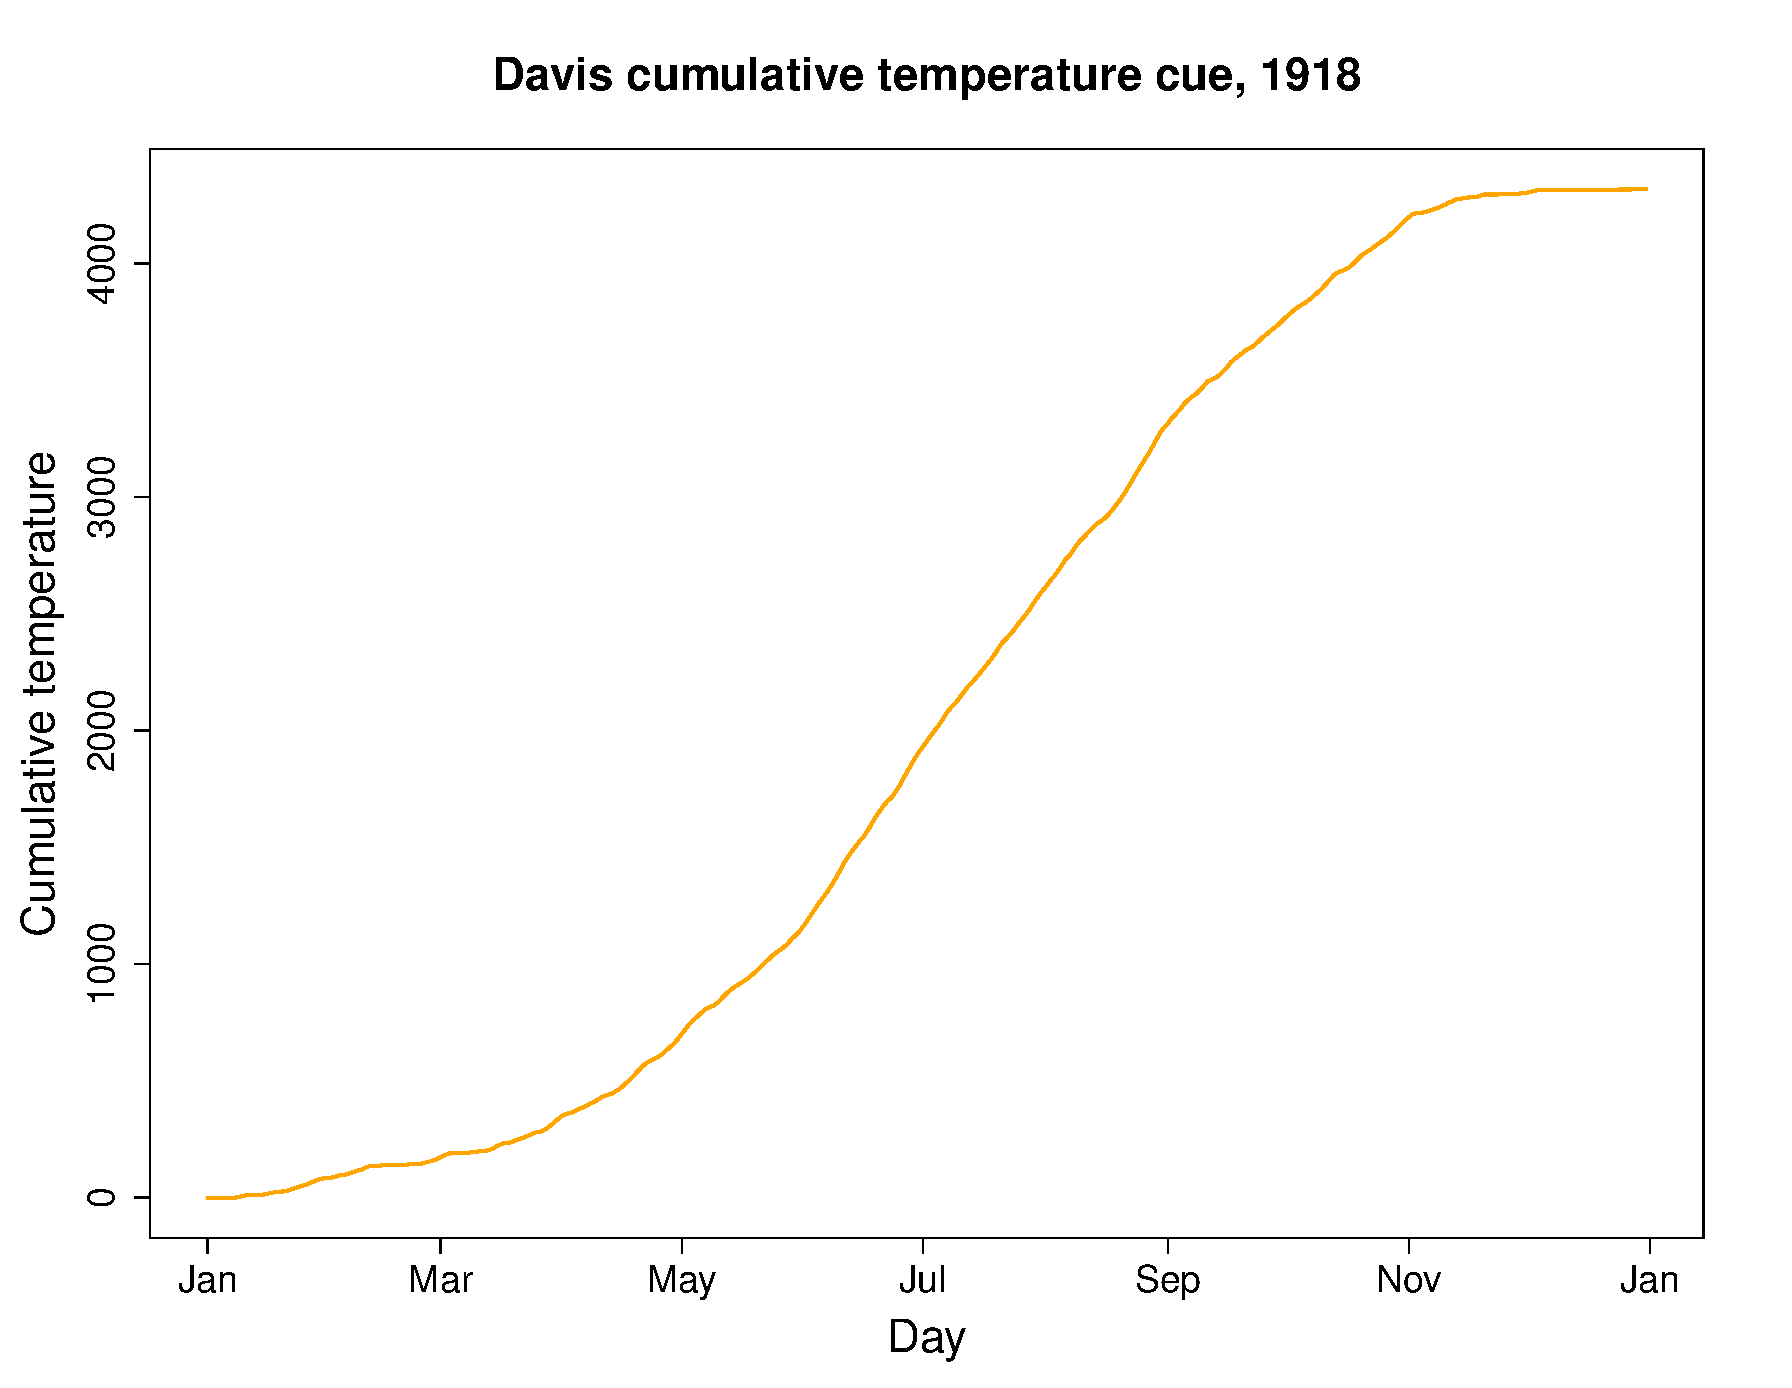
\includegraphics[width=.8\textwidth]{figs/cue-cutemp.pdf}
\end{columns}
\end{frame}

\begin{frame}
\frametitle{Emergence}
Every day, organisms combine environmental cues and traits to get an `E' value:\\
\[E=\frac{\text{photoperiod cue}}{\text{photoperiod trait}}+ \frac{\text{temperature cue}}{\text{temperature trait}}+\dots\]
If $E>1$, organism decides to emerge!
\end{frame}

\begin{frame}
\frametitle{Trait interpretation, simple example}
\begin{columns}
\column{.74\textwidth}
\only<1>{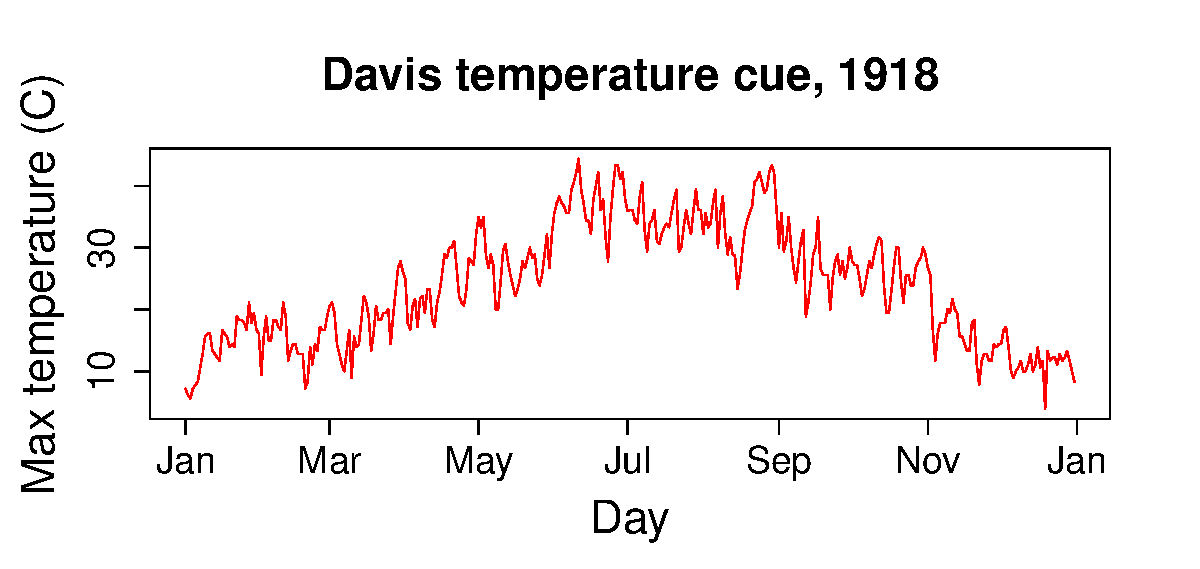
\includegraphics[width=.9\textwidth]{figs/E-example1-1.pdf}}

\only<2>{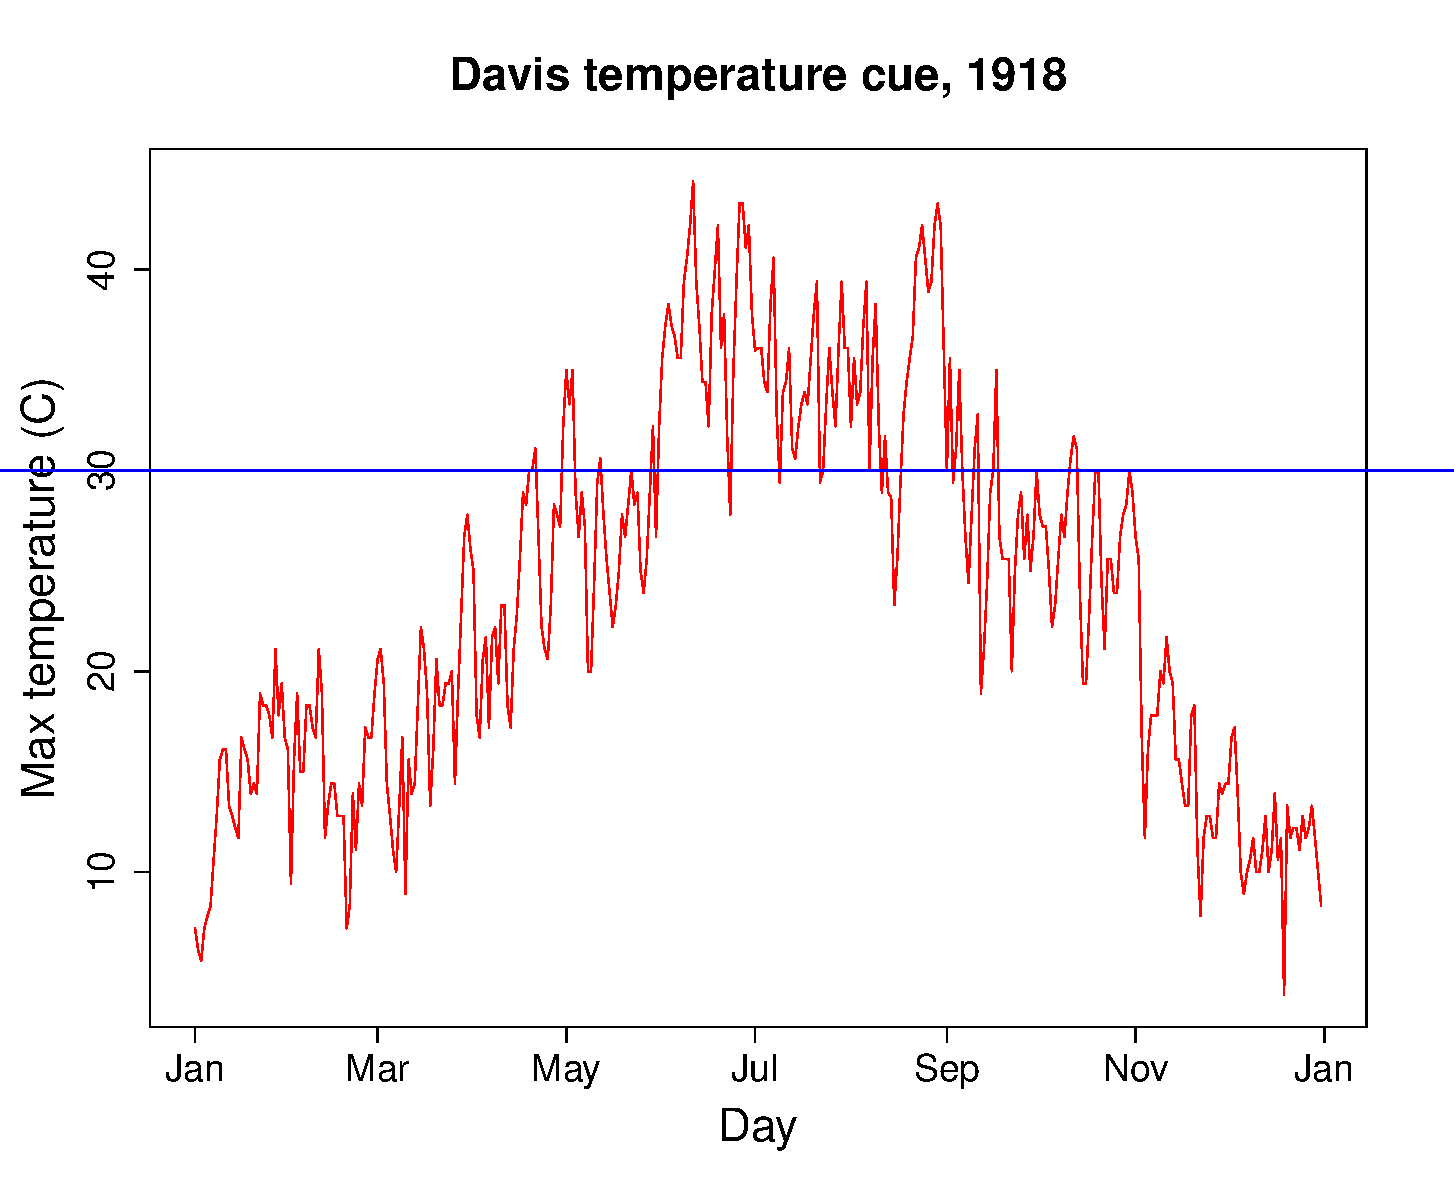
\includegraphics[width=.9\textwidth]{figs/E-example1-2.pdf}}

\only<3>{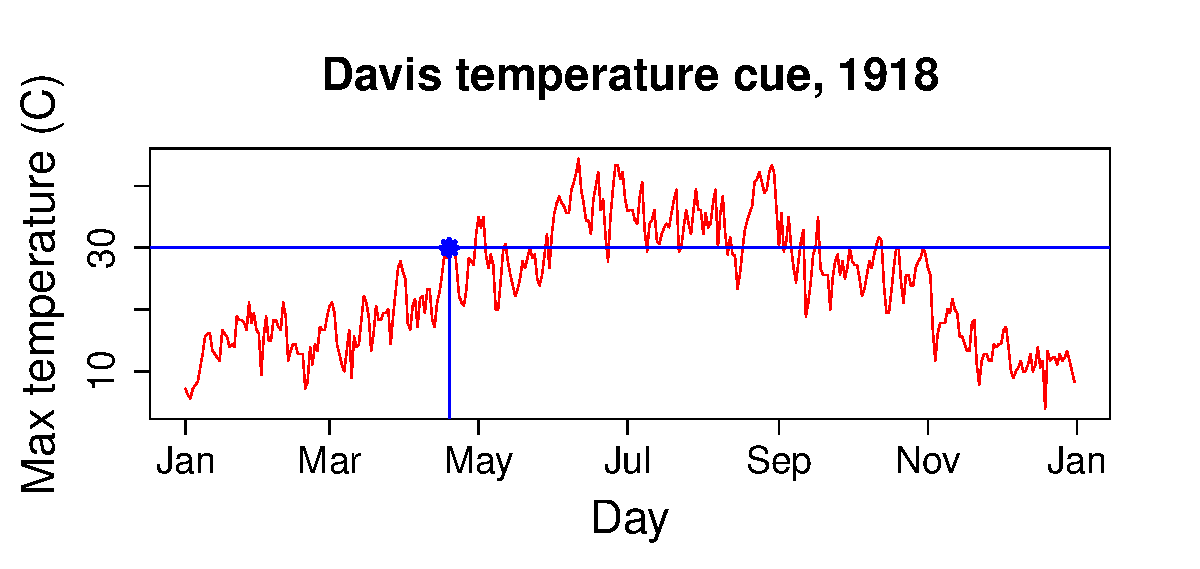
\includegraphics[width=.9\textwidth]{figs/E-example1-3.pdf}}

\column{.26\textwidth}

\begin{small}
Temp cue = 30, other cues not in use.
\end{small}
\end{columns}

\begin{tiny}
\[E=\frac{\text{temperature cue}}{30}\]
\end{tiny}
\end{frame}
%
%\begin{frame}
%\frametitle{Trait interpretation, more complex example}
%Organism relies on temp and photoperiod. Graph of the two, graph of E through time, emergence as abline
%\end{frame}

\begin{frame}
\frametitle{Fitness}
\begin{columns}

\column{.4\textwidth}
\begin{itemize}
 \item After emergence, collect resources each day (for 10 days)
 \item Daily resouces based on temp and precip
\end{itemize}

\column{.6\textwidth}

\only<2>{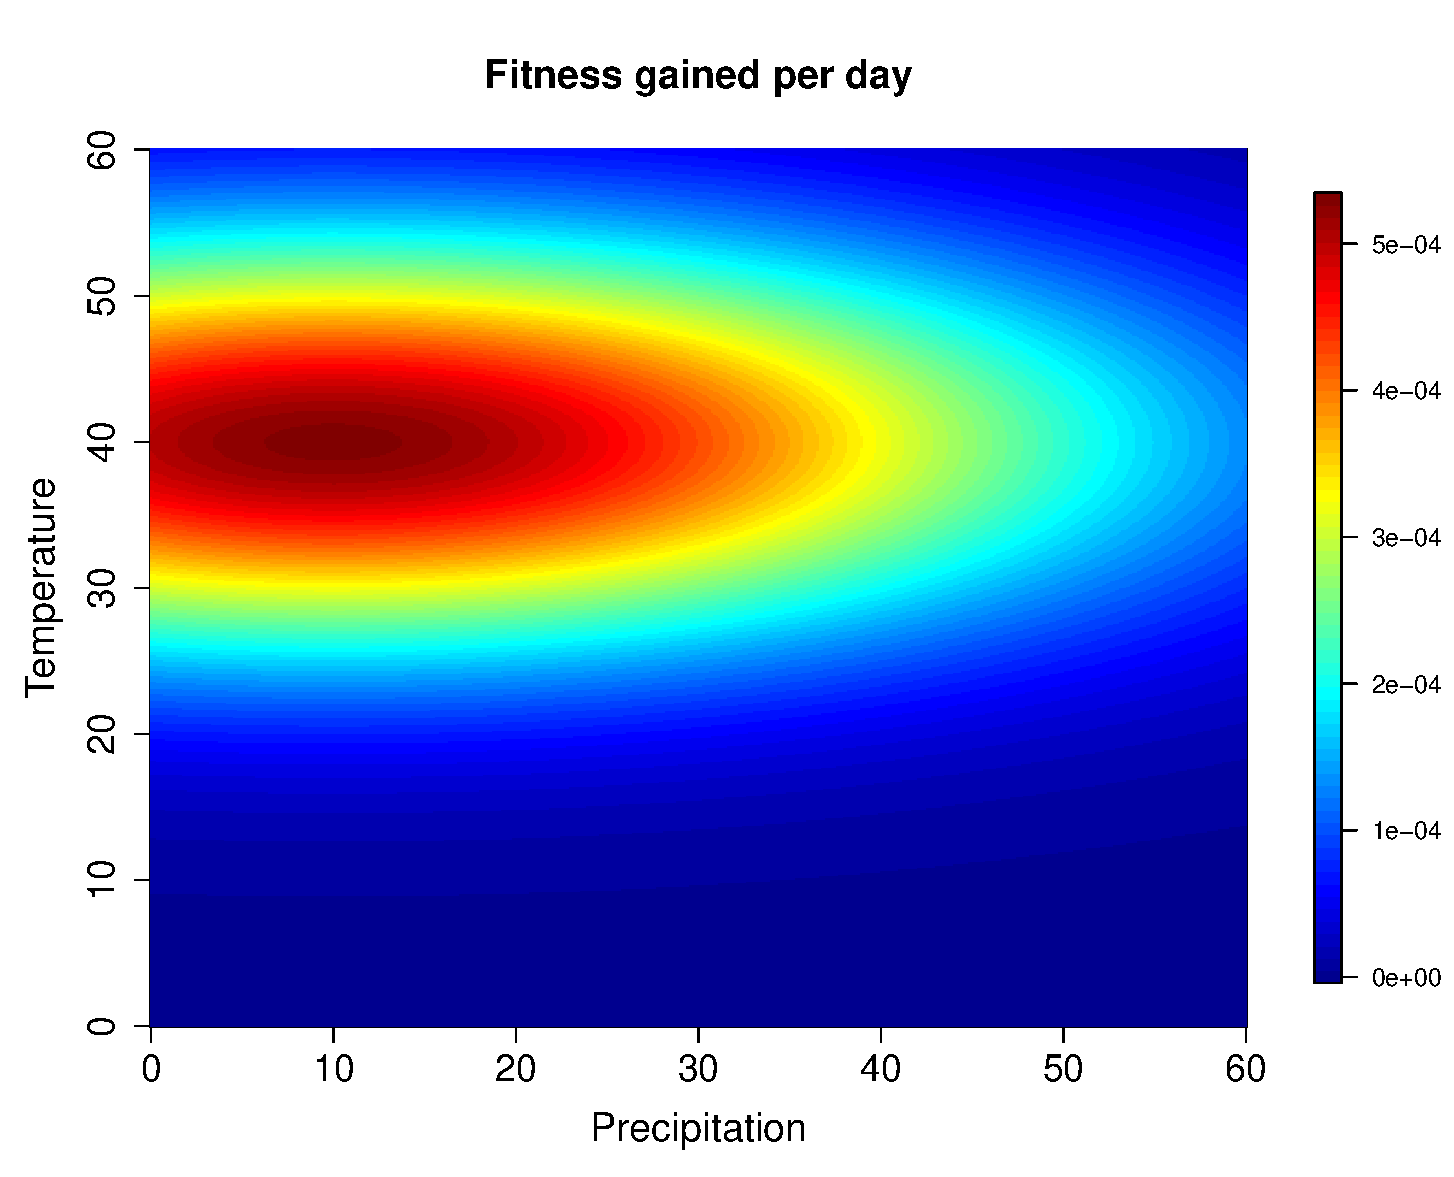
\includegraphics[width=.8\textwidth]{figs/Fitness-function.pdf}}

\only<3>{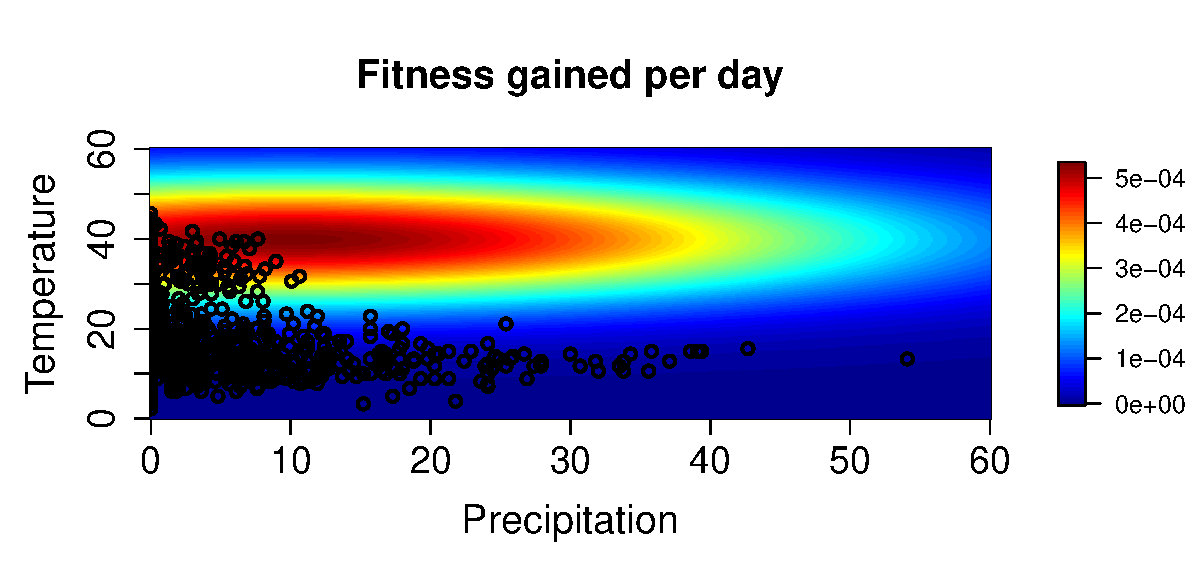
\includegraphics[width=.8\textwidth]{figs/Fitness-function-wpoints.pdf}}

\end{columns}
\end{frame}

\begin{frame}
\frametitle{Fitness}
\begin{center}

\only<1>{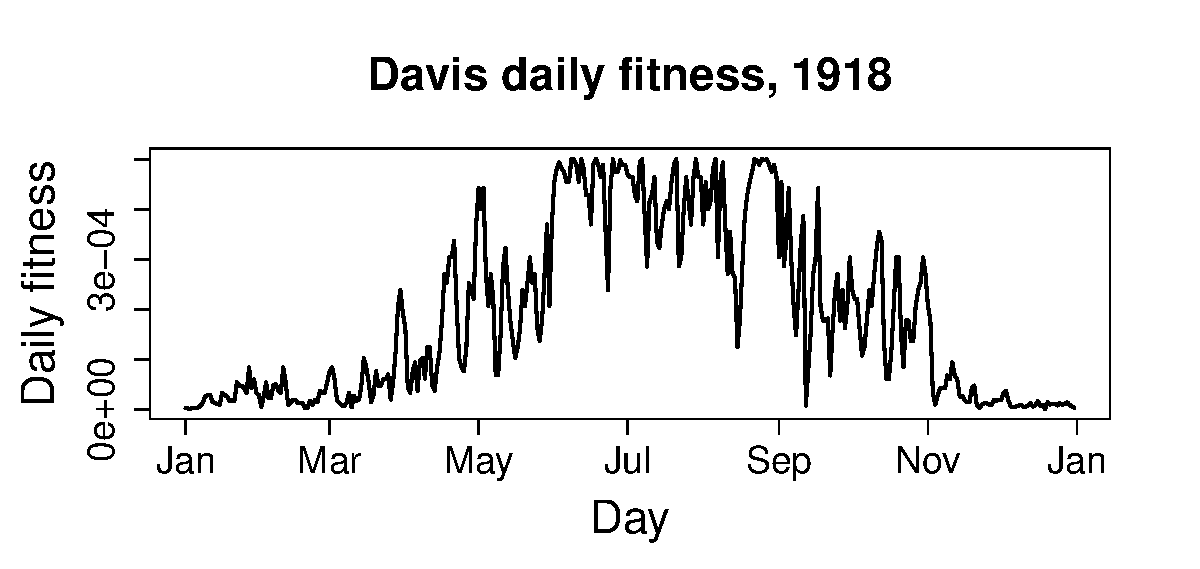
\includegraphics[width=.7\textwidth]{figs/dailyfit.pdf}}
\only<2>{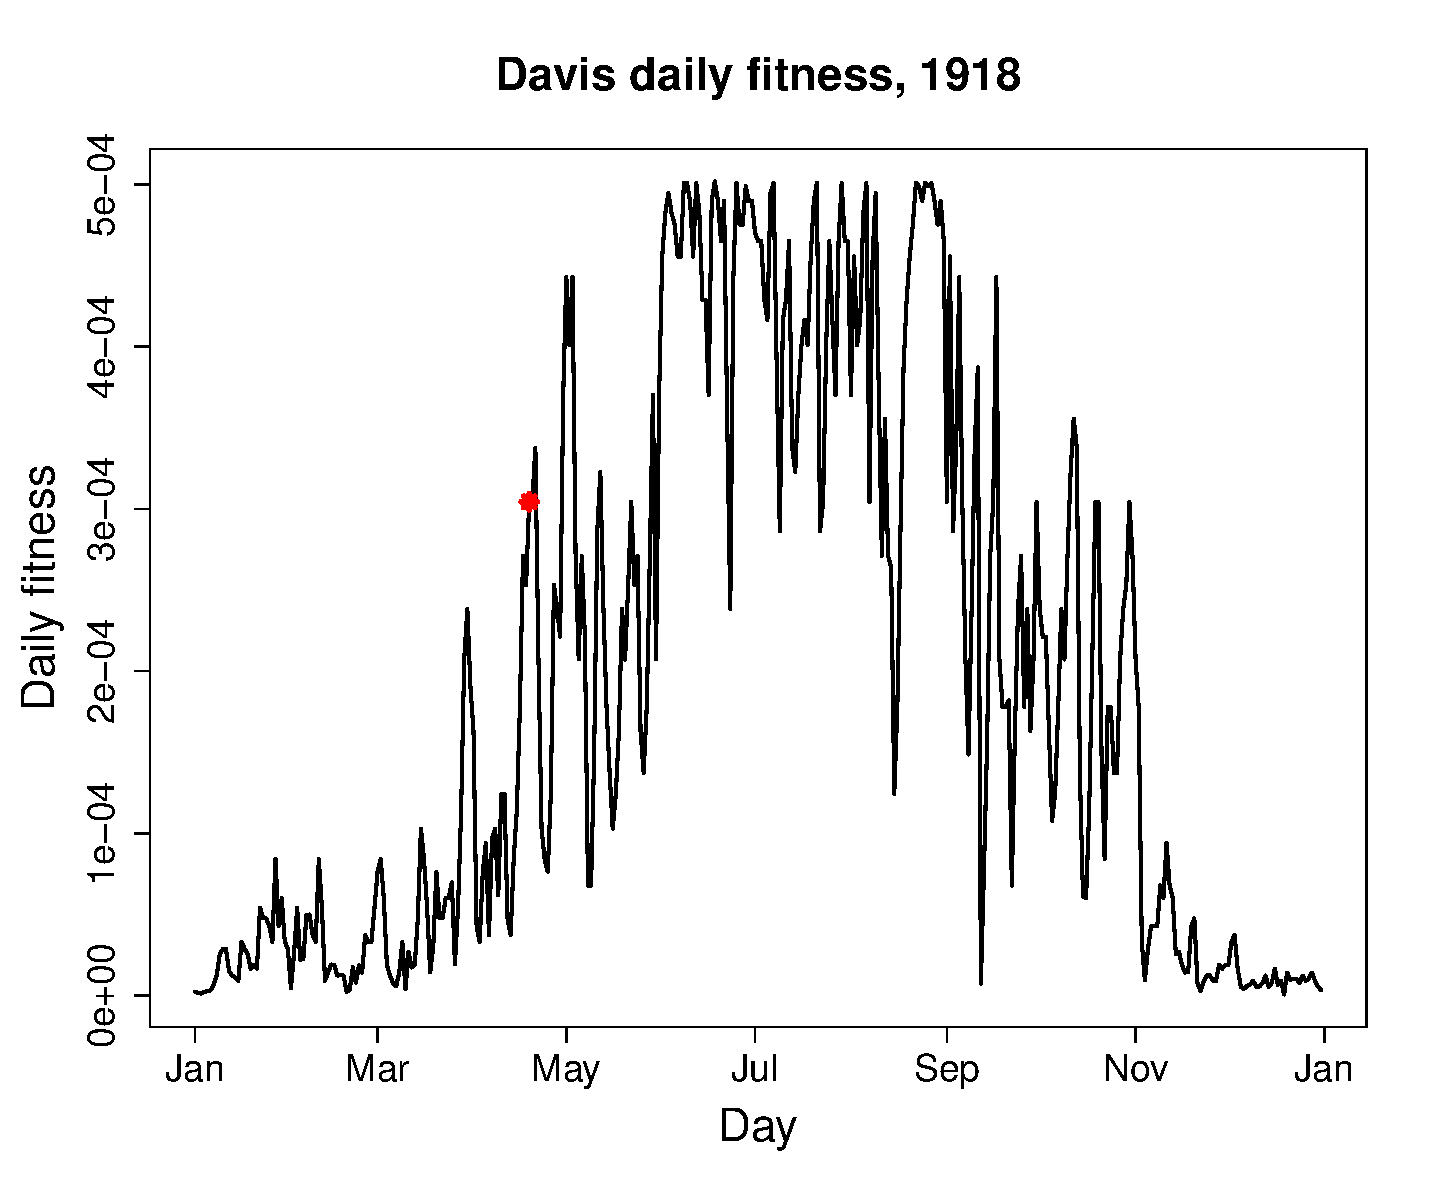
\includegraphics[width=.7\textwidth]{figs/dailyfit-2.pdf}}
\only<3>{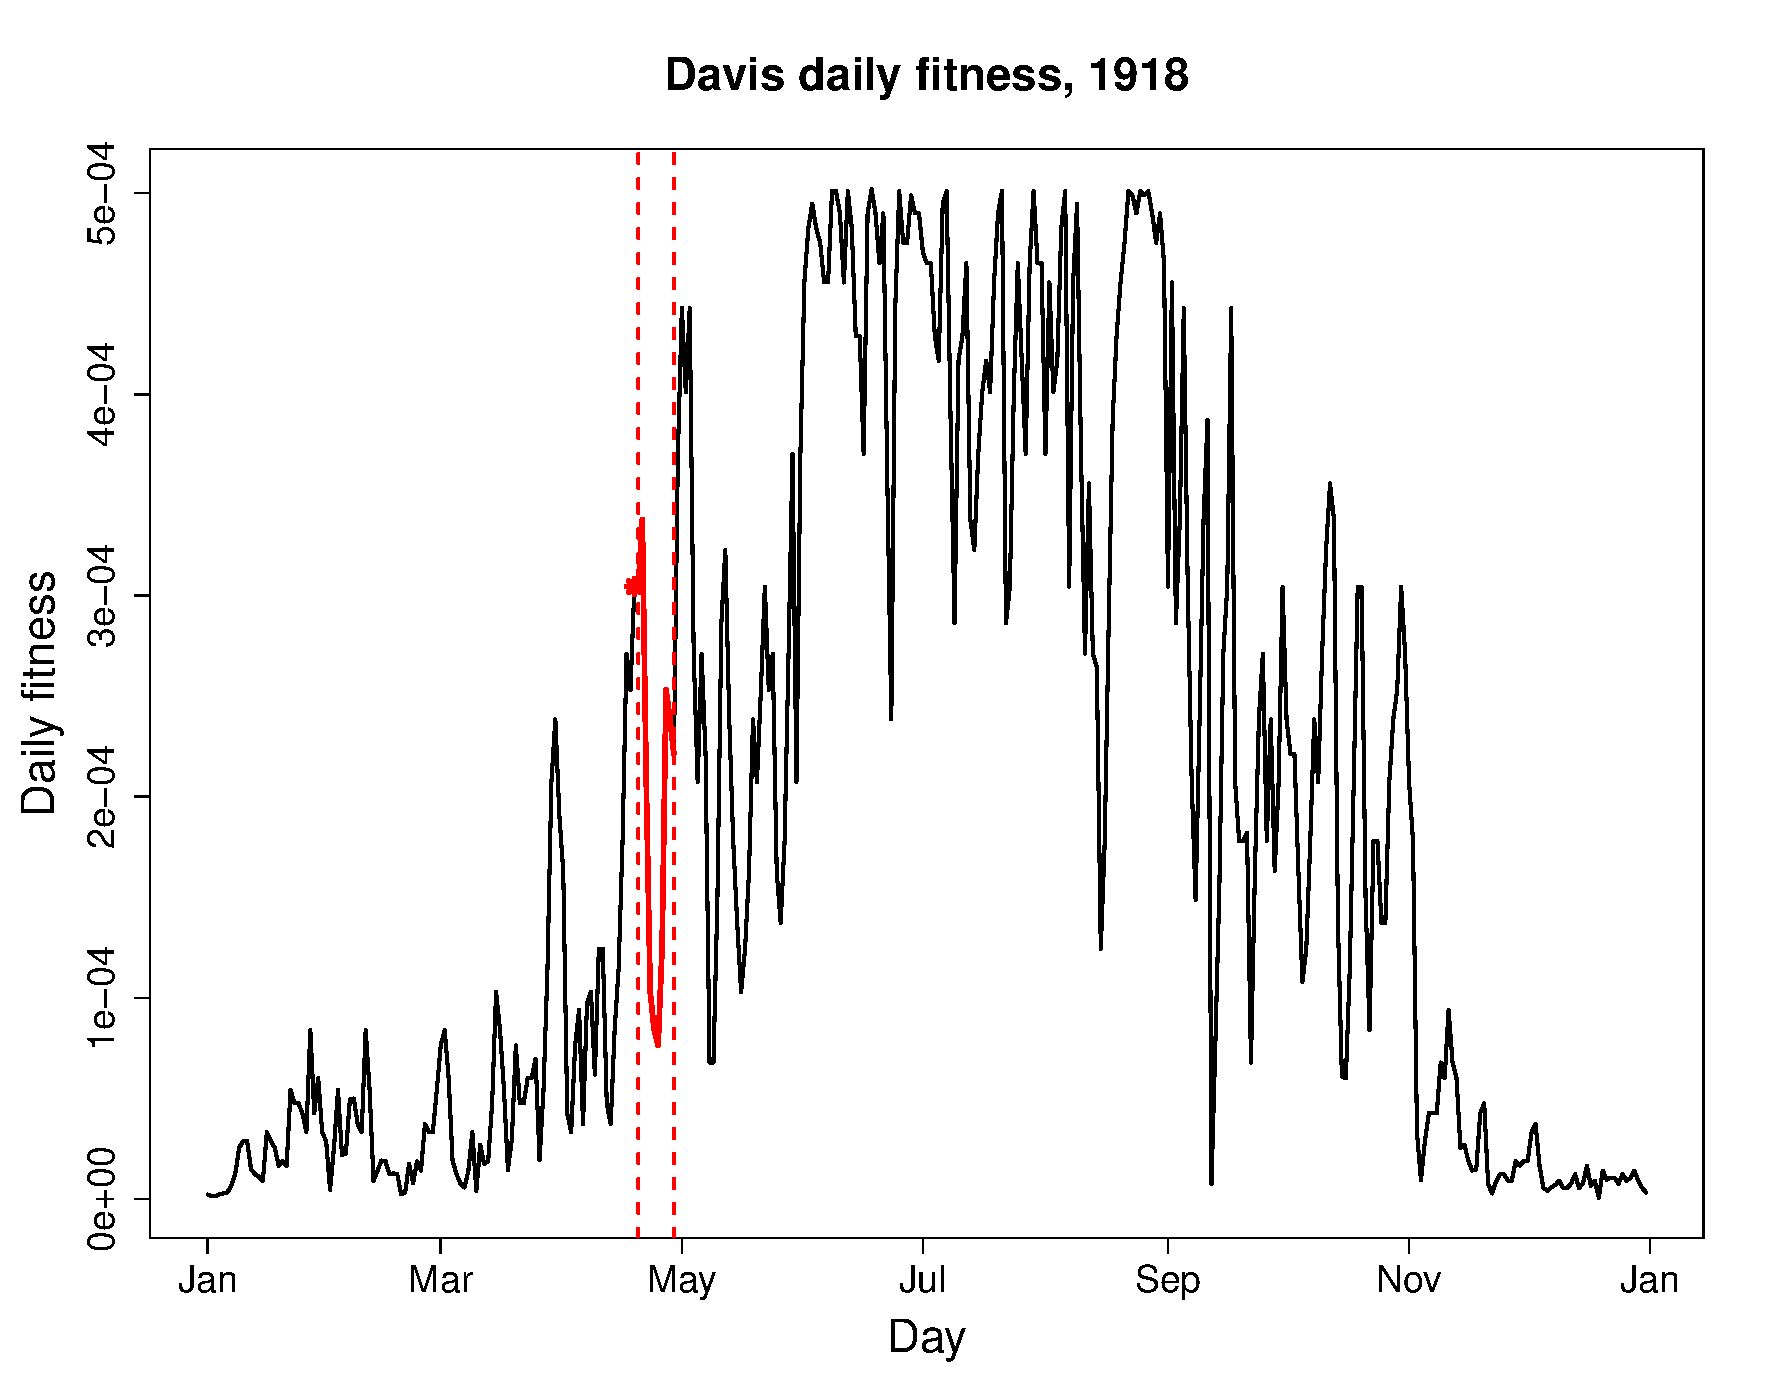
\includegraphics[width=.7\textwidth]{figs/dailyfit-3.pdf}}
\only<4>{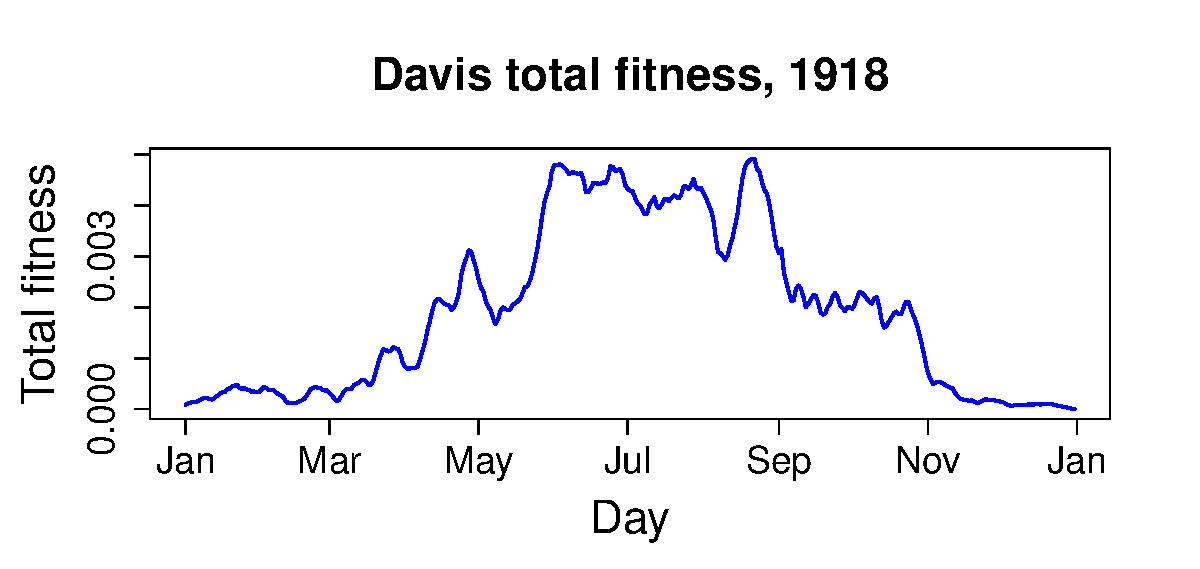
\includegraphics[width=.7\textwidth]{figs/totfit.pdf}}

\end{center}
\end{frame}


\begin{frame}
\frametitle{Reproduction: Lottery Model}

\begin{columns}
\column{.6\textwidth}
\begin{itemize}
 \item Fixed population size for all generations
 \item Assign offspring randomly proportional to fitness
 \item Offspring traits = parent + mutation (asexual)
\end{itemize}
\column{.4\textwidth}
Picture here
\end{columns}
\end{frame}

\begin{frame}
\frametitle{Simulation results}
\begin{center}
\only<1>{\includegraphics[width=.8\textwidth]{{"../../results/EEB d-t-p/resRunEEB d-t-p1/dailyfitSum-runEEB d-t-p1-gen1-actualfit"}.pdf}}
\only<2>{\includegraphics[width=.8\textwidth]{{"../../results/EEB d-t-p/resRunEEB d-t-p1/dailyfitSum-runEEB d-t-p1-gen5-actualfit"}.pdf}}
\only<3>{\includegraphics[width=.8\textwidth]{{"../../results/EEB d-t-p/resRunEEB d-t-p1/dailyfitSum-runEEB d-t-p1-gen130-actualfit"}.pdf}}
\only<4>{\includegraphics[width=.8\textwidth]{{"../../results/EEB d-t-p/resRunEEB d-t-p1/dailyfitSum-runEEB d-t-p1-gen1000-actualfit"}.pdf}}
\end{center}
\end{frame}

\begin{frame}
\frametitle{Simulation results}
\begin{center}
\only<1>{\includegraphics[width=.8\textwidth]{{"../../results/EEB d-t-p/resRunEEB d-t-p1/coefVals-b.day-b.temp-b.precip-postburn-runEEB d-t-p1"}.pdf}}
\only<2>{\includegraphics[width=.8\textwidth]{{"../../results/EEB d-t-p/resRunEEB d-t-p1/coefEffects-b.day-b.temp-b.precip-actual-postburn-runEEB d-t-p1"}.pdf}}
\end{center}
\end{frame}

\begin{frame}
\frametitle{Simulation results}
\begin{center}
{\includegraphics[width=.8\textwidth]{{"figs/coeff-eff-tern"}.pdf}}
\end{center}
%[Quaternary plots of simulations from Davis]
%[Reminder of how quaternary plots work: think of it as an NDMS plot]
%[Point to make: In this case, it looks like climate in this region (in combination with our fitness curve) has led to a fairly flat fitness peak. There are multiple strategies that work close to as well. This suggests that with the inclusion of some migration and the occasional mutation, there may be maintenance of variation in this mediterranean climate (grain of salt: fitness curve, simplicity of model)]
\end{frame}


\section{Predictive Framework}

\begin{frame}
\frametitle{Baseline year}
%One of our major goals is to make predictions for how our qualitatively different cues should be more or less valuable in climates with different levels of variation. While we want to test our simulation on other real climate regimes (in fact, we recently obtained Ithaca data), we also want to be able to manipulate the variation we're looking at [equivalent to a `lab' experiment rather than an observational one]

\begin{center}
\only<1>{\includegraphics[width=.8\textwidth]{{"figs/basyear"}.pdf}}
\only<2>{\includegraphics[width=.8\textwidth]{{"figs/basyear-plus-d2d"}.pdf}}
\only<3>{\includegraphics[width=.8\textwidth]{{"figs/basyear-plus-all"}.pdf}}
\end{center}
\end{frame}


\begin{frame}
\frametitle{Optimal traits}
\begin{center}
\vspace{-.3cm}
\only<1>{\includegraphics[width=.65\textwidth]{{"../../results/fig1/test-1000yr/winners-heatmap-run-test-1000yr"}.pdf}}
\only<2>{\includegraphics[width=.65\textwidth]{{"../../results/fig1/test-1000yr/day-by-fit-yrstd6-run-test-1000yr"}.pdf}}
\only<3>{\includegraphics[width=.8\textwidth]{{"figs/trait-response-surface"}.pdf}}
%[Because of computation limitations, haven't run numerous simulations on all combinations (YET). Instead, generated long sequence of years to represent climate, allowed organisms to use a single trait at a time, solved for the value of that trait that optimized geometric mean fitness for that climate (explicitly). Can compare how each trait alone fared for any given climate. Here we see a grid of the most useful single trait for each combination. Explain trend. BUT! This hides a lot of the real patterns]
\end{center}
\end{frame}

\begin{frame}
\frametitle{Conclusion}
\begin{columns}
\column{.3\textwidth}
\begin{tiny}
\[E=\frac{\text{photoperiod cue}}{\text{photoperiod trait}}+ \frac{\text{temperature cue}}{\text{temperature trait}}+\dots\]
\end{tiny}
\column{.3\textwidth}
\only<2-3>{\includegraphics[width=\textwidth]{{"figs/coeff-eff-tern"}.pdf}}
\column{.3\textwidth}
\only<3>{\includegraphics[width=\textwidth]{{"figs/trait-response-surface"}.pdf}}
\end{columns}
\end{frame}

\begin{frame}
\frametitle{Questions or suggestions?}
{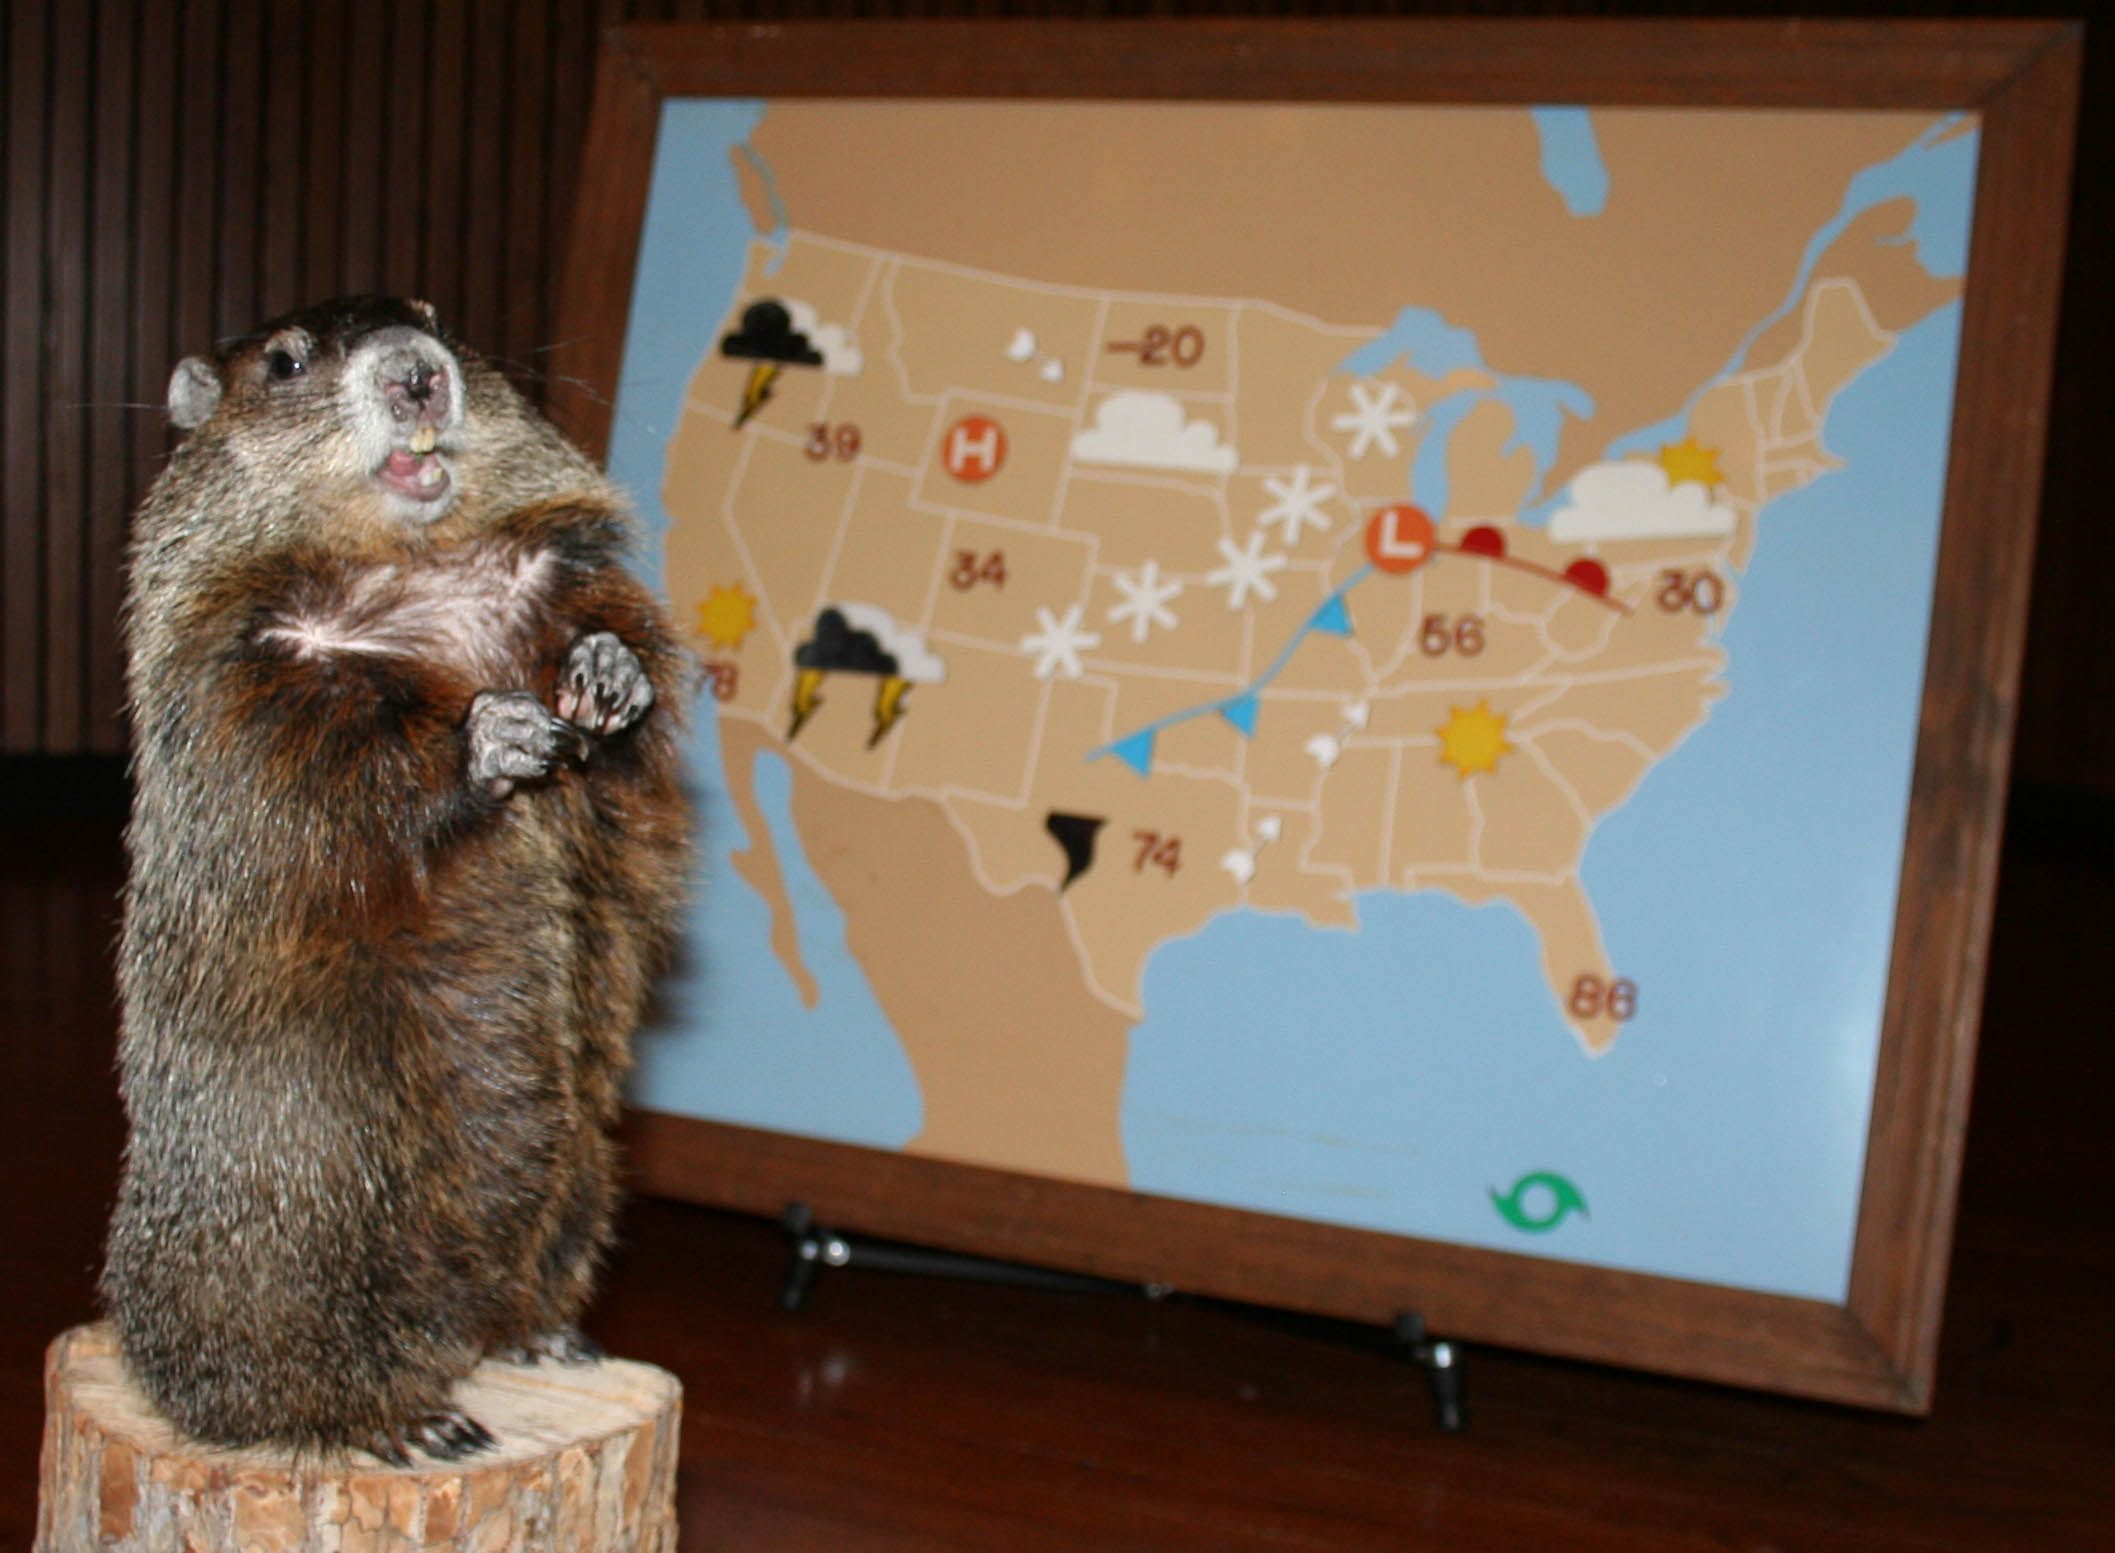
\includegraphics[width=1\textwidth]{figs/animal-weatherman.jpg}}
\end{frame}

\end{document}